\begin{document}
% ----------------------------------------
% Deckblatt
% ----------------------------------------
\newgeometry{outer=1.5cm, inner=2.5cm, top=1cm, bottom=1cm}
\thispagestyle{empty}

% ----------------------------------------
% LUH Logo                      IMKT Logo
% ----------------------------------------
\begin{tikzpicture}
    \node[anchor=south west, inner sep=0] (imkt) at (0, 0) {
        \includegraphics[width=\textwidth]{./images/imkt_logo.jpg}
    };

        \begin{scope}[x={(imkt.south east)}, y={(imkt.north west)}]
            %\draw[help lines, xstep=0.1, ystep=0.1] (0, 0) grid (1, 1);
            %\foreach \x in {0, 1, ..., 9} {
            %    \node [anchor=north] at (\x/10,0) {0.\x};
            %}
            %\foreach \y in {0, 1, ..., 9} {
            %    \node [anchor=east] at (0, \y/10,0) {0.\y};
            %}

            \node[anchor=south west, inner sep=0] (luh) at (0.1, 0.5) {
                \includegraphics[width=4cm]{./images/luh_logo.png}
            };
        \end{scope}
\end{tikzpicture}

% ----------------------------------------
% Titel der Arbeit
% ----------------------------------------
\vspace{1cm}

\begin{center}
    {\Huge Titel der Arbeit}
\end{center}

% ----------------------------------------
% Bild für diese Arbeit
% ----------------------------------------

% ----------------------------------------
% Masterarbeit und VW Logo
% ----------------------------------------
\vspace{10cm}

\begin{center}
    {\textbf{\Large Masterarbeit}}\\[1cm]

    {\large Durchgeführt bei der}

    {\Large Volkswagen AG, Wolfsburg}

    \includegraphics[width=2cm]{./images/vw_logo.png}
\end{center}

% ----------------------------------------
% Verfasser                     Betreuer
% ----------------------------------------
\begin{minipage}[t]{0.5\textwidth}
    \begin{flushleft}
        Verfasser:

        cand. mach. Ngoc Minh \textsc{Dao}
    \end{flushleft}
\end{minipage}
%
\begin{minipage}[t]{0.5\textwidth}
    \begin{flushright}
        Betreuer:

        Dipl.-Ing. Norbert \textsc{Bader}
    \end{flushright}
\end{minipage}

% ----------------------------------------
% Seperate line
% ----------------------------------------
\rule{\textwidth}{1pt}

% ----------------------------------------
% Bericht Nr                    Ort, Datum
% ----------------------------------------
\begin{minipage}[t]{0.5\textwidth}
    \begin{flushleft}
        \textbf{Bericht Nr. 1234}
    \end{flushleft}
\end{minipage}
%
\begin{minipage}[t]{0.5\textwidth}
    \begin{flushright}
        \textbf{Hannover, \today}
    \end{flushright}
\end{minipage}


\restoregeometry

% ----------------------------------------
% Table of contents
% ----------------------------------------
\tableofcontents
%\listoffigures
%\listoftables
\listoftodos[Notes]

% ----------------------------------------
% Nomenklatur
% ----------------------------------------
\addcontentsline{toc}{chapter}{Nomenklatur}
\chapter*{Nomenklatur}

\begin{longtable}{>{$}l<{$}cp{12cm}}
    \textbf{Symbol}  & \textbf{Einheit}                         & \textbf{Bezeichnung}                                         \\
    \midrule
    a                & \si{m}                                   & Halbachse der Kontaktellipse senkrecht zur Bewegungsrichtung \\
    b                & \si{m}                                   & Halbachse der Kontaktellipse parallel zur Bewegungsrichtung  \\
    C                & \si{\per\pascal}                         & Kompressibilität                                             \\
    E                & \si{\newton\per\meter^2}                 & Elastizitätsmodul                                            \\
    F                & \si{N}                                   & Normalkraft im Kontaktpunkt                                  \\
    G                & -                                        & Werkstoffparameter                                           \\
    H                & -                                        & Schmierfilmparameter                                         \\
    h                & \si{\meter}                              & Schmierfilmdicke                                             \\
    h_0              & \si{\meter}                              & Minimale Schmierfilmdicke (glatte Oberflächen)               \\
    n                & -                                        & Brechungsindex                                               \\
    P                & \si{N}                                   & Belastung im Kontakt                                         \\
    p                & \si{\pascal}                             & Druck im Kontaktpunkt                                        \\
    p_{0}            & \si{\pascal}                             & Maximaldruck im Kontaktpunkt                                 \\
    r                & \si{\meter}                              & Krümmungsradius der Kontaktkörper                            \\
    R                & \si{\meter}                              & Reziproker Krümmungsradius                                   \\
    R_{x}            & \si{\meter}                              & Hauptkrümmungsradius in der Bewegungsebene                   \\
    S                & -                                        & Schnittpunkt der Rotationsachsen                             \\
    S_{B}            & \si{\percent}                            & Bohrschlupf                                                  \\
    U                & -                                        & Geschwindigkeitsparameter                                    \\
    u                & \si[per-mode=symbol]{\meter\per\second}  & Wälzgeschwindigkeit im Schmierfilm                           \\
    W                & -                                        & Belastungsparameter                                          \\
    \alpha, \alpha^* & \si{\per\pascal}                         & Druck-Viskosität-Koeffizient                                 \\
    \beta            & \si{\per\kelvin}                         & Temperatur-Viskosität-Koeffizient                            \\
    \gamma           & \si{\per\second}                         & Schergefälle                                                 \\
    \gamma{_1}       & \si{\degree}                             & Neigungswinkel der Rotationsachse der Scheibe                \\
    \gamma{_2}       & \si{\degree}                             & Neigungswinkel der Rotationsachse der Kugel                  \\
    \eta             & \si{\pascal.\second}                     & Viskosität                                                   \\
    \eta{_0}         & \si{\pascal.\second}                     & Viskosität im Kontakteintritt ($p =$ \num{0})                \\
    \eta{_s}         & \si{\pascal.\second}                     & Viskosität beim Druck $p$ (Barus)                            \\
    \kappa           & -                                        & Verhältnis der Halbachsen der Kontaktellipsen                \\
    \nu              & -                                        & Querkontraktionszahl                                         \\
    \nu              & \si{m^2/s}                               & Kinematische Viskosität                                      \\
    \rho             & \si{kg/m^3}                              & Dichte                                                       \\
    \varphi          & \si{\degree}                             & Winkel zwischen den Hauptebenen                              \\
\end{longtable}%



% ----------------------------------------
% Einleitung
% ----------------------------------------
\chapter{Einleitung}
\label{chap:einleitung}

\section{Ziel der Arbeit}
\label{sec:ziel_der_arbeit}

\section{Vorgehensweise}
\label{sec:vorgehensweise}



% ----------------------------------------
% Stand der Technik
% ----------------------------------------
% ----------------------------------------
% Chapter: Stand der Technik
% ----------------------------------------
\chapter{Stand der Technik}
\label{chap:stand_der_technik}

Ein geschmierter Reibungskontakt kann auf vier Elemente des tribologischen Systems nach Czichos\cite{czichos} reduziert werden: Grundkörper, Gegenkörper, Zischenstoff und Umgebungsmedium.
% ----------------------------------------
% Fig: Das tribologische System
% ----------------------------------------
\begin{figure}[htb]
    \centering
    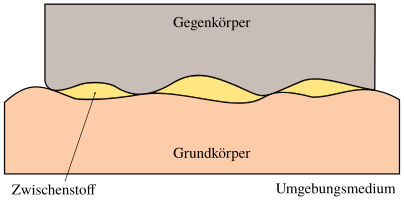
\includegraphics[]{./images/tribologisches_system.pdf}
    \caption{Das tribologische System\cite{wisniewski}}
    \label{fig:das_tribologische_system}
\end{figure}

Elastohydrodynamische Schmierung ist eine Art der Schmierung, die in der nichtkonformen Kontakt entsteht.
Diese Kontaktarten sind z.B. Wälzlager, Zahnräder, Wellendichtringe etc.
Wegen hohen Druck in der Kontaktzone werden die zu schmierende Laufflächen sich lokale verformt, daraus folgt die Erhöhung der Viskosität des Schmierstoffes.
Beide Phänomene haben eine positive Wirkung auf die Schmierfilmdicke.

Um ein besseres Verständnis der EHD-Schmierung zu haben, wird in diesem Abschnitt zuerst die Kennwerte des Zwischenstoffes (Schmiermittel) und der beiden Kontaktelementen (Grund- und Gegenkörper) ausführlich besprochen.
Danach wird der Mechanismus der EHD-Schmierung beleuchtet und am Ende wird die Arbeit von Hamrock und Dowson zur theoretischen Bestimmung der Schmierfilmdicke erwähnt.

% ----------------------------------------
% Sec: Eigenschaften des Schmiermittels
% ----------------------------------------
\section{Eigenschaften des Schmiermittels}
\label{sec:eigenschaften_des_schmiermittels}

\subsection*{Viskosität}
\label{sub:viskositaet}
Viskosität, die auch als innere Reibung bezeichnet wird, ist die wichtigste Kenngröße eines Schmierstoffes.
Sie beschreibt die Zähigkeit von Flüssigkeiten und Gasen.
Je größer die Viskosität ist, desto dickflüssiger ist das Fluid und je niedriger die Viskosität, desto dünnflüssiger ist es.
Ein Modell des Parallelplattenversuchs veranschaulicht das Fließverhalten des Schmierstoffes, Abbildung \ref{fig:geschwindigkeitsprofil_parallelplattenversuch}.
% ----------------------------------------
% Fig: Geschwindigkeitsprofil in einem Parallelplattenversuch
% ----------------------------------------
\begin{figure}[htb]
    \centering
    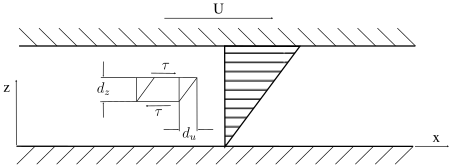
\includegraphics[]{./images/parallelplattenversuch.pdf}
    \caption{Geschwindigkeitsprofil in einem Parallelplattenversuch\cite{wisniewski}}
    \label{fig:geschwindigkeitsprofil_parallelplattenversuch}
\end{figure}

Für eine Newtonsche Flüssigkeit ist das Schergefälle $G = du/dz$ direkt proportional zur der Schubspannung $\tau$
% ----------------------------------------
% Eq: Schergefälle
% ----------------------------------------
\begin{equation}
    G = k  \tau
    \label{eq:schergefaelle}
\end{equation}

Die dynamische Viskosität (oder Viskosität) ist das Verhältnis von Schubspannung und Geschwindigkeitsgradient und ist der Kehrwert der Fluidität $k$ im Newtonschen Schubspannungsgesetz (\ref{eq:schergefaelle}).
% ----------------------------------------
% Eq: Dynamische Viskosität
% ----------------------------------------
\begin{equation}
    \eta = \frac{1}{k} = \frac{\tau}{G} = \frac{\tau}{du/dz}
    \label{eq:dynamische_viskositaet}
\end{equation}

Die kinematische Viskosität ergibt sich aus der dynamischen Viskosität durch die Division mit der Dichte des Fluids.
% ----------------------------------------
% Eq: Dynamische Viskosität
% ----------------------------------------
\begin{equation}
    \nu = \frac{\eta}{\rho}
    \label{eq:kinematische_viskotitaet}
\end{equation}

Im Si-Einheitensystem hat die dynamische Viskosität als Einheit $N  s/m^2$ oder $Pa  s$ und die kinematische Viskosität als Einheit $m^2/s$.
Ein Stoff hat die Viskosität $1~N  s/m^2$, wenn er in zwischen zwei Platten, die Größe von $1~m^2$ und einen Abstand von $1~m$ haben, befindet und man braucht $1~N$, um die zwei Platten gegeneinander mit einer Geschwindigkeit von $1~m/s$ zu verschieben.

\subsection*{Temperatureffekt}
\label{sub:temperatureffekt}
Die Temperatur hat eine große Effekt auf der Viskosität aller fließfähigen Stoffe.
Mit steigender Temperatur sinkt die Viskosität der Flüssigkeiten ab.
Diese Effekt kann experimentell mittel eines Viskosimeters und rechnerisch nach Cameron bestimmt werden.

Die einfachste Gleichung nach Reynold lautet:
% ----------------------------------------
% Eq: Dynamische Viskosität nach Reynold
% ----------------------------------------
\begin{equation}
    \eta = \eta_{s}  \ exp \left( -\beta  \Delta\phi \right)
    \label{eq:dynamische_viskositaet_reynold}
\end{equation}
%
wobei $\eta_{s}$ ist die Viskosität des Schmierstoffes bei der Temperatur $\phi_{s}$, $\eta$ ist die Viskosität des Schmierstoffes bei der Temperatur $\phi$, $\Delta{\phi}$ ist die Temperaturdifferenz ($\eta = \eta_{s} + \Delta{\phi}$) und $\beta$ ist die thermoviskose Konstante.\improvement{check the formel}
% ----------------------------------------
% Eq: Dynamische Viskosität nach Cameron
% ----------------------------------------
\begin{equation}
    \eta(\phi) = k_1  \ exp \left( k_2 / (\phi + 95) \right)
    \label{eq:dynamische_viskositaet_cameron}
\end{equation}

\subsection*{Viskositätsindex}
\label{sub:Viskositaetsindex}
Die Temperaturabhängigkeit der kinematischen Viskosität eines Schmieröls wird auch von einem Viskositätsindex (VI oder KVI) beschreibt.
Der Viskositätsindex basiert auf einer Skalar, in der zwei unterschiedlichen Öltypen mit deutlich abweichenden Viskosität-Temperaturverhalten zugeordnet wurden.
Das Öl, das starke Veränderung der Viskosität ist, wird mit 0 oder LVI (low viscosity index) indiziert.
Das andere Öl wird mit 100 oder HVI (high viscosity index) gekennzeichnet.
Aus dem Vergleich der kinematischen Viskosität eines zu beschreibenden Öls mit diesen beiden Referenzölen bei $100^\circ$  ergibt sich dessen Viskositätsindex, Formel \ref{eq:viskositaetsindex}.
% ----------------------------------------
% Eq: Viskositätsindex
% ----------------------------------------
\begin{equation}
    VI~(oder KVI) = \frac{\nu_0 - \nu}{\nu_0 - \nu_{100}}
    \label{eq:viskositaetsindex}
\end{equation}
%
In der VI-Definition ist es angenommen, dass die Veränderung der Viskosität mit Temperatur von drei Ölen linear ist.
Die Linearisierung ist nach Walther\cite{walther} und wird in der Abbildung~\ref{fig:variation_der_viskositaet_mit_temperatur} für das Mineralöle dargestellt.
% ----------------------------------------
% Fig: Naeherungsgleichung der Viskosität-Temperatur nach Walther
% ----------------------------------------
\begin{figure}[htb]
    \centering
    \includegraphics[width=5cm]{./images/blank_img.jpg}
    \caption{Variation der Viskosität mit Temperatur}
    \label{fig:variation_der_viskositaet_mit_temperatur}
\end{figure}

\subsection*{Einfluss von Druck auf Viskosität}
\label{sub:einfluss_von_druck_auf_viskositaet}
Mit steigendem Druck nimmt die Viskosität aller Schmieröle zu.
% ----------------------------------------
% Fig: Viskosität - Druck - Verhalte
% ----------------------------------------
\begin{figure}[htb]
    \centering
    \includegraphics[width=5cm]{./images/blank_img.jpg}
    \caption{Dynamische Viskosität in Abhängigkeit vom Druck}
    \label{fig:dynamische_viskositaet_in_abhaengigkeit_vom_druck}
\end{figure}
%
Allerdings verändert sich das Schmiermittel unter dem für die EHD-Kontakte enormen Druck schlagartig.
Die Viskosität nimmt rapide zu und der Schmierstoff erreicht einem festen Zustand.
Nach Barus kann die Viskosität mit der unteren Formel berechnet werden
% ----------------------------------------
% Eq: Viskositätsindex
% ----------------------------------------
\begin{equation}
    \eta = \eta_0 \ exp(\alpha_p  p)
    \label{eq:dynamische_viskositaet_druck_barus}
\end{equation}
%
wobei $\eta_0$ die Viskosität beim Atmosphärendruck und $\alpha_p$ der Druckkoeffizient der Viskosität ist.
Für Mineralöle sind diese Parameter ungefähr
\begin{align*}
    0,001 \leq \ &\eta_0 \leq 0,1 \quad Pas \\
    0 \leq \ &\alpha \leq 4,0 \times 10^{-8} \quad Pa^{-1}
\end{align*}
%
Leider liefert die Barus Gleichung einen zu großen Wert beim hohen Druck.
Eine genauer Gleichung wurde von Roelands\cite{roelands} vorgeschlagen
% ----------------------------------------
% Eq: Roelands Gleichung
% ----------------------------------------
\begin{equation}
    \eta(p, T) = \eta_0 \ exp \left[ (\ln{\eta_0} + 9,67)
                              \left( \left( 1 + \frac{p}{p_r} \right) ^z 
                              \left( \frac{T_0 - 138}{T - 138} \right)^{s_0} -1 \right) \right]
    \label{eq:dynamische_viskositaet_druck_roelands}
\end{equation}
%

Der Druckkoeffizient der Viskosität $\alpha_p$ ist nicht eine Konstante, sondern eine Funktion der Temperatur.
Diese Abhängigkeit wird in Abbildung~\ref{fig:druckkoeffizient_temperatur} für die Referenzöle der FVA gezeigt.
% ----------------------------------------
% Fig: Druckkoeffizient der FVA-Referenzöle in Abhängigkeit von der Temperatur
% ----------------------------------------
\begin{figure}[htb]
    \centering
    \includegraphics[width=5cm]{./images/blank_img.jpg}
    \caption{Verhalten des Druckkoeffizienten in Abhängigkeit von der Temperatur}
    \label{fig:druckkoeffizient_temperatur}
\end{figure}
%

\subsection*{Dichte}
\label{sub:dichte}

Für eine numerische Schmierfilmdickenmessung ist es notwendig zu wissen, wie die Dichte des Schmierstoffes unter verschiedenen Druck verhält.
Die Form des Schmierfilms kann nicht richtig berechnet werden, wenn diese Eigenschaft vernachlässigt wird.
Die Kompressibilität eines Schmierstoffes $C$ ist nach Chu und Cameron mit folgender Formel zu berechnen:
% ----------------------------------------
% Eq: Die Kompressibilität eines Schmierstoffes
% ----------------------------------------
\begin{equation}
    \label{eq:kompressibilitaet}
    C = \left( \frac{1}{\rho} \right) \frac{d\rho}{dp} = \left( \frac{1}{V} \right) \frac{dV}{dp}
\end{equation}
%
wobei V das Volumen und $dV$ die Änderung des Volumens ist.

Die Dichte der Mineralöle ist nach Hirano\cite{hirano} mit folgender Formel zu berechnen
% ----------------------------------------
% Eq: Dichte nach Hirano
% ----------------------------------------
\begin{equation}
    \label{eq:dichte_hirano}
    \rho = \rho_0 \left( 1 + \frac{0,6  p}{1 + 1,7  p} \right)
\end{equation}
%
wobei $p$ in $GPa$ und $\rho_0$ die Dichte beim normalen Luftdruck ($0,87~kg/m^3$ bei $20^\circ C$) ist.
% ----------------------------------------
% Fig: Druckkoeffizient der FVA-Referenzöle in Abhängigkeit von der Temperatur
% ----------------------------------------
\begin{figure}[htb]
    \centering
    \includegraphics[width=5cm]{./images/blank_img.jpg}
    \caption{Variation der Dichte bei verschiedenen Drücke}
    \label{fig:variation_der_dichte_bei_verschiedenen_druecke}
\end{figure}

\subsection*{Brechungsindex}
\label{sub:brechungsindex}

Für die Messverfahren, die auf optischen Interferometrie basieren, braucht man die Abhängigkeit zwischen der Dichte und dem Brechungsindex des Schmierstoffes.
Nach Gohar wird das Verhältnis mit der Formel\ref{eq:dichte_brechnungsindex} beschrieben.
% ----------------------------------------
% Eq: Dichte und Brechungsindex
% ----------------------------------------
\begin{equation}
    \label{eq:dichte_brechnungsindex}
    c  p = \frac{n^2 - 1}{n^2 + 2}
\end{equation}
%
wobei $c$ ein Ölkonstante ist (zB: SAE30, $c = 0,33$).
Der Brechungsindex für meist Mineralöle bei normalen Luftdruck ist c.a 1,51.


\subsection*{Wärmeleitfähigkeit}
\label{waermeleitfaehigkeit}

Um die Temperaturerhöhung des Schmierstoffes unter Schubspannung zu schätzen, ist dessen Wärmeleitfähigkeit $k$ nötig.
Nach Cameron\cite{cameron} kann diese Größe beim normalen Luftdruck mit folgender Formel berechnet werden.
% ----------------------------------------
% Eq: Wärmeleitfähigkeit
% ----------------------------------------
\begin{equation}
    \label{eq:waermeleitfaehigkeit}
    k = \frac{0,1173 - 6,33 \times 10^{-5} \ T}{\rho_0}
\end{equation}
%
wobei $T$ die absolute Temperatur in $K$ und $\rho_0$ die Dichte in $kg/m^3$ ist.

\subsection*{Newtonsche Fluide}
\label{sub:newtonsche_fluide}

Wenn die Viskosität eines Fluids von der Schubspannung unabhängig ist, wird das Fluid als newtonsches Fluid bezeichnet - Abbildung\ref{fig:newtonsche_fluide}.
Flüssigkeiten, deren Viskosität mit steigender Schubspannung zunimmt, nennt man dilatant.
Solches Verhalten ist geeignet für Suspensionen, nicht als Schmierstoff.
Strukturviskose Fluide sind die Umkehr der Dilatanz.
Strukturviskosität tritt bei synthetischen Fluiden auf.
Für die Bestimmung der Schmierfilmdicke werden alle Fluide in Rahmen dieser Arbeit als newtonsche Fluide angenommen.
% ----------------------------------------
% Fig: Newtonsche und nicht newtonsche Fluide
% ----------------------------------------
\begin{figure}[htb]
    \centering
    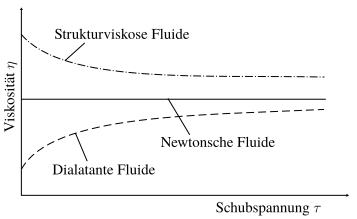
\includegraphics[]{./images/newtonsche_nichtnewtonsche_fluide.pdf}
    \caption{Newtonsche und die andere Fluide\cite{wisniewski}}
    \label{fig:newtonsche_fluide}
\end{figure}
%

% ----------------------------------------
% Sec: Betrachtung des EHD-Kontaktes
% ----------------------------------------
\section{Betrachtung des EHD-Kontaktes}
\label{sec:betrachtung_des_ehd_kontaktes}

Die Kontaktflächen von Maschinenelementen werden in zwei Grundformen eingeteilt.
Dies sind konforme (z.B. Gleitlager) und nichtkonforme Paarungen (z.B. Zahnrad, Reibrad, Nocken-Stößel).
Abbildung~\ref{fig:nichtkonforme_kontakte} zeigt die Beispiele konforme und nichtkonforme Kontakte.
% ----------------------------------------
% Fig: Nichtkonforme Paarungen
% ----------------------------------------
\begin{figure}[htb]
    \centering
    \includegraphics[width=5cm]{./images/blank_img.jpg}
    \caption{Nichtkonforme Kontakte}
    \label{fig:nichtkonforme_kontakte}
\end{figure}
%
Gegenteil zu den konformen Kontakten, wo die Pressungen in der Größenordnung von $10 MPa$ auftreten, können in zwischen den Laufflächen nichtkonformer Kontakt die Druckspannungen 0,5 GPa und höher betragen.
Durch die enorme, konzentrierte Belastung werden die Flächen an dem Kontaktpunkt elastisch verformt und vergrößert.
Im Folgenden soll der Wälzkontakt nach Wisniewski\cite{wisniewski} näher betrachtet werden.

\subsection*{Kontakt von beliebig gekrümmten Elementen}
\label{sub:kontakt_von_beliebig_gekruemmten_elementen}

Bei der Betrachtung des konzentrischen Kontaktes werden alle Oberflächen als ideal glatt angenommen und durch deren minimalen und maximalen Krümmungen wird die Geometrie des Grundkörpers bzw. des Gegenkörpers beschrieben.
Beim konvexen Körper (Index 1) sind die Krümmungsradien ($r_{11}, r_{12}$) positiv und beim konkaven Körper (Index 2) sind die Radien ($r_{21}, r_{22}$) negativ.
Zwischen den beiden Ebenen, die $r_{11}$ und $r_{21}$ erhalten, bildet sich der Winkel $\varphi$.
In Abbildung~\ref{fig:kontaktgeometrie_nichtkonforme_kontakte} wird die generelle Kontaktgeometrie bei nicht konformen Festkörpern dargestellt.
% ----------------------------------------
% Fig: Wälzkontakt nach Wisniewski
% ----------------------------------------
\begin{figure}[htb]
    \centering
    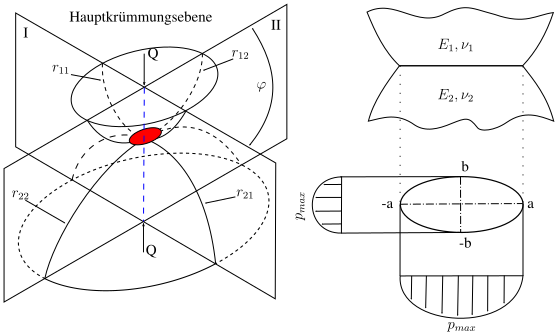
\includegraphics[]{./images/Hertzsche_Pressung.pdf}
    \caption{Kontaktgeometrie bei nicht konformer Paarungen\cite{psm}}
    \label{fig:kontaktgeometrie_nichtkonforme_kontakte}
\end{figure}
%
Im Kontaktpunkt bildet sich die Kontaktflächen eine Ellipse mit den Halbachsen $a$ und $b$.
Zu $a$ und $b$ zu bestimmen, braucht man das reduzierte Elastizitätsmodul $E$, die Belastung $P$ und der Krümmungsradius $R$.
% ----------------------------------------
% Eq: Laengen der Halbachsen der Kontaktellipse
% ----------------------------------------
\begin{align}
    a = \beta_a  \sqrt[3]{\frac{3  P  R}{E}} \label{eq:laenge_a} \\
    b = \beta_b  \sqrt[3]{\frac{3  P  R}{E}} \label{eq:laenge_b}
\end{align}
%
Der reduzierte Elastizitätsmodul $E$ beschreibt die elastische Eigenschaften der beiden Elemente und wird definiert als
% ----------------------------------------
% Eq: Der reduzierte Elastizitätsmodul E
% ----------------------------------------
\begin{equation}
    \label{eq:reduzierter_elastizitaetsmodul}
    \frac{1}{E} = \frac{1}{2}  \left( \frac{1 - \nu_1^2}{E_1} + \frac{1 - \nu_2^2}{E_2} \right)
\end{equation}
%
wobei $\nu_x$ die Querkontraktionszahl der Kontaktkörper und $E_x$ der Elastizitätsmodul der Kontaktkörper ist.
Die Druckverteilung $p$ hat eine Form eines Halbellipsoids und wird so definiert
% ----------------------------------------
% Eq: Druckverteilung p
% ----------------------------------------
\begin{equation}
    \label{eq:druckverteilung}
    p = p_0  \sqrt{1 - \left( \frac{x}{b} \right)^2 - \left( \frac{y}{a} \right)^2}
\end{equation}
%
wobei $x, y$ die Koordinaten in der Ebene und die maximale Pressung $p_0$ ein Produkt der Belastung $P$ und der Länge von Halbachsen $a, b$ sind.
% ----------------------------------------
% Eq: Maximale Pressung p0
% ----------------------------------------
\begin{equation}
    \label{eq:maximale_pressung}
    p_0 = \frac{3  P}{2  \pi  a  b}
\end{equation}
%
Der reziproke Krümmungsradius $R$ wird mit der Summe aller vier Hauptkrümmungen $r_x$ bestimmt
% ----------------------------------------
% Eq: Krümmungsradius R
% ----------------------------------------
\begin{equation}
    \label{eq:kruemmungsradius}
    \frac{1}{R} = \frac{1}{r_{11}} + \frac{1}{r_{12}} + \frac{1}{r_{21}} + \frac{1}{r_{22}}
\end{equation}
%
Die Koeffizienten $\beta_a$ und $\beta_b$ zur Bestimmung der Berührungsfläche in einem konformen Kontakt kann über den Parameter $\cos{\psi}$ aus dem Diagram~\ref{fig:beta_a_und_beta_b_als_funktion_der_cos_psi} abgelesen werden.
% ----------------------------------------
% Fig: beta_a und beta_b als Funktion des cos_psi
% ----------------------------------------
\begin{figure}[htb]
    \centering
    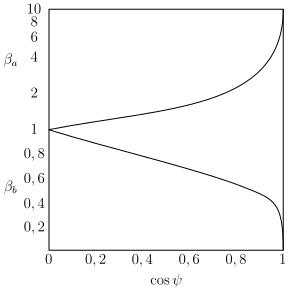
\includegraphics[]{./images/beta_cos_psi_diagram.pdf}
    \caption{$\beta_a$ und $\beta_b$ als Funktion von $\cos{\psi}$\cite{wisniewski}}
    \label{fig:beta_a_und_beta_b_als_funktion_der_cos_psi}
\end{figure}
%

Der Parameter $\cos{\psi}$ kann mit folgender Formel\ref{eq:cos_psi} berechnet werden
% ----------------------------------------
% Eq: cos psi
% ----------------------------------------
\begin{equation}
    \label{eq:cos_psi}
    \cos{\psi} = R  \sqrt{\left( \frac{1}{r_{11}} - \frac{1}{r_{12}} \right)^2 
                                + \left( \frac{1}{r_{21}} - \frac{1}{r_{22}} \right)^2 
                                + 2  \cos{2 \varphi} 
                                 \left( \frac{1}{r_{11}} - \frac{1}{r_{12}}  \right)^2 
                                 \left( \frac{1}{r_{21}} - \frac{1}{r_{22}} \right)^2}
\end{equation}
%

Für ein Kugel-Scheibe-Modell gilt
%
\begin{align*}
    r_{11} &= r_{12} = r_{Kugel} \\
    r_{21} &= r_{22} = r_{Scheibe} = \infty
\end{align*}
%
Eingesetzt diese Werte in \ref{eq:kruemmungsradius} und in \ref{eq:cos_psi} ergibt sich 
%
\begin{align*}
    R &= r_{Kugel}/2 \\
    \cos{\psi} &= 0
\end{align*}
%
Aus dem Diagramm für den Fall $\cos_{\psi} = 0$ liefert den Wert $\beta_a = \beta_b = 1$.
Werden diese in die \ref{eq:laenge_a} und \ref{eq:laenge_b} eingesetzt, ergibt sich
%
\begin{align*}
    a = b
\end{align*}
%
Damit ist es bewiesen, dass hier ein kreisförmiger Kontakt vorliegt.

\subsection*{Kontakt von rauhen Festkörpern}
\label{sub:kontakt_von_rauhen_festkoerpern}
In Realität können die Oberflächen der Kontaktkörper nie perfekt glatt sein.
Da die Mikrogeometrie der Kontaktkörper den Einfluss auf die Abmessungen der Kontaktzone bzw. auf die Bestimmung der maximalen Pressungen hat, ist eine einfache Anwendung der vorherigen Studie von glatten Festkörpern für die rauhe Oberflächen nicht geeignet.
Zum Vergleich mit den glatten Oberflächen sind bei rauhen Festkörpern die Kontaktflächen größer und dadurch sind die maximalen Pressungen kleiner - Abbildung\ref{fig:druckverteilung_beim_glatten_und_rauhen_kontakt}
% ----------------------------------------
% Fig: Druckverteilung im konzentrischen Kontakt, glatten und rauhen
% ----------------------------------------
\begin{figure}[htb]
    \centering
    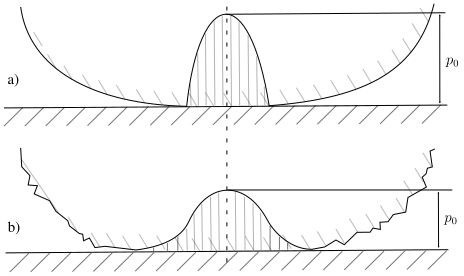
\includegraphics[]{./images/druckverteilung_im_konzentrierten_kontakt.pdf}
    \caption{Druckverteilung beim glatten (a) und rauhen (b) Kontakt\cite{wisniewski}}
    \label{fig:druckverteilung_beim_glatten_und_rauhen_kontakt}
\end{figure}
%

\subsection*{Kontakt von beschichteten Festkörpern}
\label{sub:kontakt_von_beschichteten_Festkoerpern}
\improvement[inline]{blah blah blah}

% ----------------------------------------
% Sec: Elastohydrodynamische Schmiertheorie
% ----------------------------------------
\section{Elastohydrodynamische Schmiertheorie}
\label{elastohydrodynamische_schmiertheorie}

Erklärung, wie EHD funktioniert

% ----------------------------------------
% Sec: Schmierung nach Hamrock und Dowson
% ----------------------------------------
\section{Schmierfilmdicke nach Hamrock und Dowson}
\label{sec:schmierfilmdicke_nach_hamrock_und_dowson}
Erklärung, wie mann die Schmierfilmdicke berechnen kann



% ----------------------------------------
% Literaturforschung der experimentellen Technik in der EHD Schmierung
% ----------------------------------------
\chapter{Literaturforschung der experimentellen Techniken zur Schmierfilmdickenmessung in EHD-Kontakten}
\label{chap:literaturforschung_der_experimentellen_technik_in_ehd_schmierung}
% ----------------------------------------
% Optische Methode
% ----------------------------------------
\section{Optische Messung der EHD Schmierfilmdicke}
\label{sec:optische_messung_der_ehd_schmierfilmdicke}

\subsection{Licht Interferometrie}
\label{ssec:licht_interferometrie}

\subsection{Variante von der klassichen optischen Interferometrie Methode}
\label{ssec:variante_interferometrie}

% ----------------------------------------
% Elektrische Methode
% ----------------------------------------
\section{Elektrische Messung der EHD Schmierfilmdicke}
\label{sec:elektrische_messung_der_ehd_schmierfilmdicke}

\subsection{Kapazitive Methoden}
\label{ssec:kapazitive_methoden}

\subsection{Resistive Methoden}
\label{ssec:resistive_methoden}

% ----------------------------------------
% Alternative Methoden
% ----------------------------------------
\section{Alternative EHD Schmierfilmdicke Messmethoden}
\label{sec:alternative_messmethoden}

\subsection{Ultraschall}
\label{ssec:ultraschall}

\subsection{Laserinduzierte Fluoreszenz}
\label{ssec:laserinduzierte_fluoreszenz}


% ----------------------------------------
% Aufbau und Funktion des EHD-Messgeräts
% ----------------------------------------
% ----------------------------------------
% Chap: Aufbau und Funktion des EHD-Messgeräts
% ----------------------------------------
\chapter{Aufbau und Funktion des EHD-Messgeräts}
\label{chap:aufbau_und_funktion_des_ehd_messgeraets}

Zur Schmierfilmdickenmessung wurde ein ``EHL Ultra Thin Film Measurement System'' der Firma PCS-Instrument genutzt (Abbildung \ref{fig:ehl_messgeraet}).
Basiert auf dem Kugel-Scheibe-Modell und optischer Interferenz wird die Schmierfilmdicke im EHD-Kontakt ermittelt.
Durch einen leicht modifizierten Aufbau, ermöglicht das Gerät auch die Bestimmung von Reibkoeffizienten der eingesetzten Schmierstoffe.
Im Folgenden wird kurz auf die einzelnen Komponenten des EHL-Gerätes und die Modifikation im Rahmen dieser Arbeit eingegangen.

% ----------------------------------------
% Fig: EHL Prüfstand
% ----------------------------------------
\begin{figure}[htb]
    \centering
    \includegraphics[width=0.8\linewidth]{./images/ehl_pruefstand.png}
    \caption{EHL-Messgerät \cite{ehl}}
    \label{fig:ehl_messgeraet}
\end{figure}

% ----------------------------------------
% Sec: PC und Elektronikeinheit
% ----------------------------------------
\section{PC und Elektronikeinheit}
\label{sec:pc_elektronikeinheit}

Zur Bedienung des Prüfstands steht einen PC zur Verfügung.
Der PC hat Windows 98 als Betriebssystem und fünf ISA-Steckkarten.
Diese Karten sind für die Ein-/Ausgabe, die Zeiterfassung, die SW-Bilderfassung sowie ADC und DAC zuständig.
Die Kommunikation mit dem Prüfstand erfolgt durch das Softwarepaket ``Ultra Thin Film EHL Measurement''.
Der PC ist mit einem Spektrometer, einem SW-Monitor und einer Elektronikeinheit verbunden.

Zu der Elektronikeinheit gehören die Motoren, die Lasteinheit sowie die Heizvorrichtung.
Außerdem ist eine Überwachungsfunktion eingebaut, die beim einem Absturz der Software oder des PC den Prüfstand abschaltet.

% ----------------------------------------
% Sec: Meschanischer Aufbau
% ----------------------------------------
\section{Mechanischer Aufbau}
\label{sec:mechanischer_aufbau}

Abbildung \ref{fig:ehl_aufbau} zeigt den Schematischen Aufbau des EHL-Prüfstands.
Das Reservoir ist bei Messungen mit Öl bis die Hälfte der Kugel gefüllt.
Durch die Heizvorrichtung kann das Öl bis c.a \SI{150}{\degreeCelsius} temperiert werden.
% ----------------------------------------
% Fig: EHL Aufbau
% ----------------------------------------
\begin{figure}[htb]
    \centering
    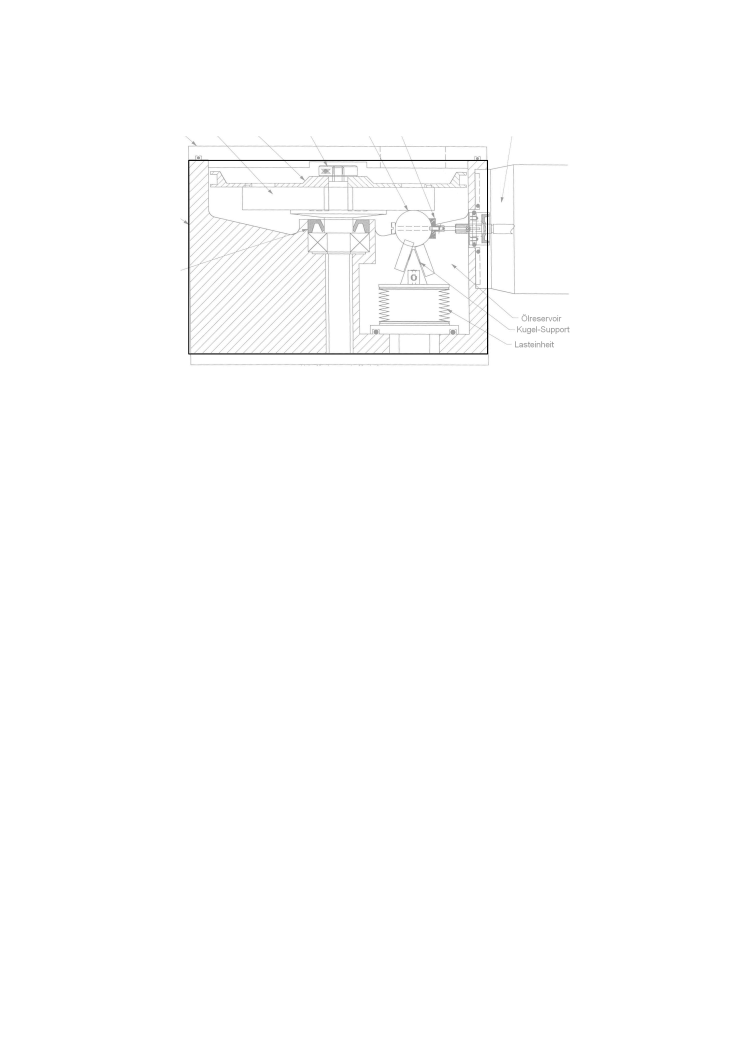
\includegraphics[width=0.8\textwidth]{./images/ehd_pruefstand_aufbau.pdf}
    \caption{Schematischer Aufbau des EHL-Prüfstands \cite{ehl}}
    \label{fig:ehl_aufbau}
\end{figure}
%
Der elastohydrodynamische Schmierfilm wird durch einen Kugel-Scheibe-Kontakt erzeugt.
Die Kugel ist hochglanzpoliert, aus 100Cr6 Stahl und hat einen Durchmesser von \SI{19.05}{\milli\meter}.
Es gibt zwei Variationen der Kugel, normal und durchgebohrt.
Über ein Kugel-Support wird die Kugel von unten von eine Lasteinheit gegen einer sich rotierenden Glasscheibe gedrückt.
Die Last ist von \SIrange{0}{50}{\newton} wählbar und ergibt sich einen maximalen Druck von \SI{0.7}{\giga\pascal} im Kontaktpunkt.
Die Glasscheibe hat einen Durchmesser von \SI{100}{\milli\meter} und ist an der Unterseite mit einer durchlässigen Chromschicht und einer Silikatschicht zu versehen.
Es gibt insgesamt \num{21} befahrbaren Spuren (R = $34 \rightarrow 44$ \si{\milli\meter}) auf der Scheibe durch die axiale Verschiebung des Kugel-Supports.
Ein Spurwechsel ist nötig, weil die Silikatschicht, die nicht so robust sowie die Chromschicht ist, mit Laufe der Zeit abgenutzt wird.

Die Glasscheibe kann von \SI{1}{\milli\meter\per\second} bis \SI{5}{\meter\per\second} durch einen Motor betrieben werden.
Ein weiterer Motor ermöglicht auch das Antreiben der Kugel.
In diesem Fall sind Versuche mit Schlüpf zwischen Kugel und Scheibe innerhalb von \SIrange{0}{200}{\percent} ermöglicht.

Das originale Kugel-Support von PCS-Instrument besteht aus drei Lager, die auf einem dreieckigen Aluminium-Klotz geschraubt werden.
Eine modifizierte Lagerung mit einstellbarer, geführte Achse von Wittek \cite{wittek_2007} steht auch zur Verfügung (Abbildung \ref{fig:kugel_support}).
% ----------------------------------------
% Fig: Kugel-Support
% ----------------------------------------
\begin{figure}[htb]
    \centering

    \begin{subfigure}[b]{0.3\textwidth}
        \includegraphics[width=\textwidth]{./images/kugel-support_original.png}
    \end{subfigure}
    %
    \begin{subfigure}[b]{0.3\textwidth}
        \includegraphics[width=\textwidth]{./images/kugel-support_wittek.png}
    \end{subfigure}
    \caption{Originaler PCS-Support (links) und modifizierter Support (rechts) \cite{wittek_2007}}
    \label{fig:kugel_support}
\end{figure}
%

In Tabelle \ref{tab:ehl_specs} sind die wichtigsten Daten zu dem Prüfstand zusammengefasst.
% ----------------------------------------
% Table: EHL Prüfstand Spezifikationen
% ----------------------------------------
\begin{table}[h]
    \centering
    \caption{EHL-Prüfstand Spezifikationen}
    \begin{tabular}{m{5cm}L}
        \multicolumn{2}{l}{\textbf{Kugel}} \\
        Material & Stahl (100Cr6) \\
        Durchmesser & \phi 19.05 \ mm \\
        Rauheit Rq & 0.0235 \ \mu m \\

        \hline

        \multicolumn{2}{l}{\textbf{Glasscheibe}} \\
        Material & Glas \\
        Durchmesser & \phi 100 \ mm \\
        Rauheit Rq & 0.033 \ \mu m \\
        Spuren & 21 \\
        Befahrbarer Radius & 34 \rightarrow 44 \ mm \\
        Beschichtung & Chrom, Silikat \\

        \hline

        \multicolumn{2}{l}{\textbf{Motoren}} \\
        Geschwindigkeit & 1 \ mm/s \rightarrow 5 \ m/s \\
        Geschwindigkeit Sprung & 0 \rightarrow 100 \% \\
        Schlupf (Kugel-Scheibe) & 0 \rightarrow 200 \% \\

        \hline

        \multicolumn{2}{l}{\textbf{Belastung}} \\
        Last & 0 \rightarrow 50 \ N \\
        max. Pressung & 1.1 \ GPa \ (Stahl), 0.7 \ GPa \ (Glas) \\

        \hline

        \multicolumn{2}{l}{\textbf{Ölreservoir}} \\
        Volumen & 120 \ ml \\
        Temperierung & T_{Raum} \rightarrow 150^\circ C \\

        \hline

        \multicolumn{2}{l}{\textbf{Messsystem}} \\
        Schmierfilmdicke & 0 \rightarrow 1000 \ nm \\
        Genauigkeit & \pm 1 \ nm \\
    \end{tabular}
    \label{tab:ehl_specs}
\end{table}


% ----------------------------------------
% Sec: Messsystem zur Schmierfilmdickemessung
% ----------------------------------------
\section{Messsystem zur Schmierfilmdickemessung}
\label{sec:messsystem_zur_schmierfilmdickemessung}

Beim EHD-Prüfstand von PCS Instrument wird die Schmierfilmdicke im Kugel-Scheibe-Kontakt mit Weißlichtinterferometrie (siehe Abschnitt \ref{sec:optische_messung_der_ehd_schmierfilmdicke}) bestimmt.
Der Kontakt wird von oben durch das Glasscheibe beleuchtet und das zurück reflektierende Bild wird von einem Spektrometer bewertet.
Die Messeinrichtung wird in Abbildung \ref{fig:ehl_messprinzip} angezeigt.
% ----------------------------------------
% Fig: EHL Messeinrichtung
% ----------------------------------------
\begin{figure}[htb]
    \centering
    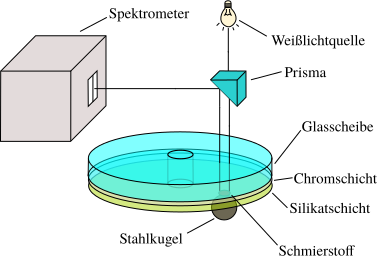
\includegraphics[]{./images/ehd_messprinzip.pdf}
    \caption{Messprinzip des EHD-Prüfstand von PCS \cite{mach_2008}}
    \label{fig:ehl_messprinzip}
\end{figure}
%

Die Glasscheibe hat nicht nur eine Chromschicht, sondern auch eine Silikatschicht (Spacer-Layer) darauf.
Die hat eine Funktion sowie ein Hart-Ölfilm, der immer da ist, das heißt es auch beim Stillstand die Interferenzen gibt.
Interferenzmuster im Auge des Betrachters sind fabelhafte Bilder (Abbildung \ref{fig:ehl_bilder}) und aus ihrer Farben kann die Schmierfilmdicke bei bekannter Silikatschictdicke berechnet werden.
% ----------------------------------------
% Fig: EHL Interferenzbilder
% ----------------------------------------
\begin{figure}[htb]
    \centering
    \includegraphics[width=0.8\textwidth]{./images/ehl_contact_at_increasing_speeds.png}
    \caption{Interferenzmuster eines Punktkontaktes bei zunehmenden Geschwindigkeiten \cite{ehl_broshure}}
    \label{fig:ehl_bilder}
\end{figure}
%

Da eine Auswertung der Schmierfilmdicke aus den Farben der Interferenzen durch einen Beobachter zu ungenau wäre, wird der zurück reflektierende Lichtstrahl über einen Prisma durch einen Spalt in ein Spektrometer geleitet.
Dort werden die Interferenzmuster analysiert und an einem SW-Monitor angezeigt (Abbildung \ref{fig:ehl_interferenzmuster}).

% ----------------------------------------
% Fig: EHL Beugungsmuster
% ----------------------------------------
\begin{figure}[htb]
    \centering
    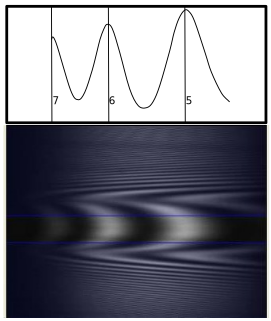
\includegraphics[]{./images/interferenzsmuster.pdf}
    \caption{Interferenzmuster im Spektrometer \cite{ehl_broshure}}
    \label{fig:ehl_interferenzmuster}
\end{figure}
%
Der senkrechte, weiße Balken im Interferenzmuster sind die Maxima, wo die konstruktive Interferenzen stattfinden, und die gibt dabei die Wellenlänge an.
Wandern diese Balken nach rechts, nimmt die Wellenlänge bzw. Schmierfilmdicke zu.
Mit Hilfe des Ultra-Softwarepakets kann man aus dem Interferenzmuster die genaue Schmierfilmdicke berechnen.



% ----------------------------------------
% Konstruktive Bearbeitung
% ----------------------------------------
% ----------------------------------------
% Chap: Konstruktive Bearbeitung
% ----------------------------------------
\chapter{Konstruktive Bearbeitung}
\label{chap:konstruktive_bearbeitung}

Um die Messgenauigkeit der optischen Interferometrie-Technik mit der einfachen Adaptierbarkeit an verschiedenen realen Maschinenelementen der elektrischen Messmethode zur Schmierfilmdickenmessung im EHD-Kontakt zu vereinigen, soll ein neues modular Messsystem auf Basis des EHD-Prüfstands von PCS entwickelt werden.
Dies System soll die optische und elektrische (kapazitive) Messung gleichzeitig erlauben.
Für solches System gibt es die folgende Anforderungen, die durch konstruktive Bearbeitung in nächsten Abschnitten gelöst werden.
\begin{itemize}
    \item Elektrische Isolierung der Glasscheibe und der Kugel mit dem gesamten System.
    \item Elektrische Zugänge für die Messproben an der Scheibe und der Kugel.
    \item Beschichtung auf der Scheibe, die elektrische und optische Messung gleichzeitig erlaubt.
\end{itemize}

% ----------------------------------------
% Sec: Konstruktion der Kugelführung
% ----------------------------------------
\section{Konstruktion der Kugelführung}
\label{sec:konstruktion_der_kugelfuehrung}

Da das modifizierte Kugelsupport mit einstellbarer Achse von \textit{E. Wittek} \cite{wittek_2007} wegen Rundlaufabweichung nur bis Wälzgeschwindigkeit von c.a 0,7 $m/s$ einsetzbar ist, wird die originale Kugelführung der PCS Firma im Rahmen dieser Arbeit modifizierte und weiter benutzt.
Bei der standardmäßigen Kugelführung wird eine durchgebohrte Kugel in einem Adapter eingeklemmt, welche dann über einen Querstift mit der Motorausgangswelle des zweiten Antriebs formschlüssig verbunden wird.
Für die kapazitive Messung soll die Kugel elektrisch mit dem gesamten System isoliert werden, das erfolgt durch die Verwendung eine Kunststoffwelle.
Die Kugelaufnahme wird aus Messing gefertigt, um den Kontaktwiderstand mit den zu Signal übertragenden Kohlebürsten zu reduzieren.
Die Abbildung \ref{fig:aufbau_der_neuen_kugelfuehrung} zeigt den Zusammenbau der neuen Kugelführung.
% ----------------------------------------
% Fig: Aufbau der neuen Kugelführung
% ----------------------------------------
\begin{figure}[htb]
    \centering
    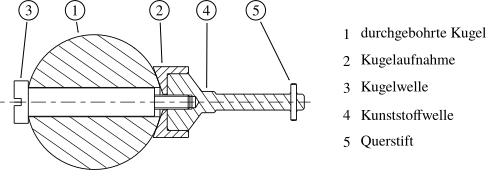
\includegraphics[]{./images/durchgebohrte_kugel.pdf}
    \caption{Aufbau der neuen Kugelführung}
    \label{fig:aufbau_der_neuen_kugelfuehrung}
\end{figure}
%

Die geführte Kugelachse ermöglicht die Versuche mit Schlupf und verhindert auch das unkontrollierte Einbringen des Schmierstoffes (Öl, Fett) in den Kontakt.
Der Kraftfluss zwischen dem zweiten Motor und der Kugel kann durch den Wegfall des Querstifts unterbrochen werden.
In diesem Fall dreht sich die Kugelführung frei in der Motorausgangswelle.

% ----------------------------------------
% Sec: Konstruktion des Kugelsupports
% ----------------------------------------
\section{Konstruktion des Kugelsupports}
\label{sec:konstruktion_des_kugelsupports}

Das neue Kugelsupport besteht aus drei Rillenkugellager, die durch drei $M3$ Schrauben auf einem dreieckigen Sockel befestigt werden (Abbildung \ref{fig:das_modifizierte_kugelsupport}).
Die Kugel wird von den drei Lagern sicher von unten gegen der Glasscheibe gestützt.
Da die Kugel mit der Lasteinheit elektrisch isoliert werden muss, wird der Sockel aus Kunststoff gefertigt.
Auf der Unterseite des Sockels befinden sich zwei Löcher, die mit den Stifte der Lasteinheit arretiert werden, dadurch wird die Position des Kugelsupports während Versuche sicher gestellt.
An der Seite des Sockels sind zwei M3 Bohrung zur Anbringung der Kohlebürstenhalter, die für die Aufnahme der elektrischen Signale von der Kugel zuständig sind, zu versehen.
Bei der Versuchen mit Fett ist dort auch möglich, die Befettungsvorrichtung zu montieren.
% ----------------------------------------
% Fig: Das modifizierte Kugelsupport
% ----------------------------------------
\begin{figure}[htb]
    \centering
    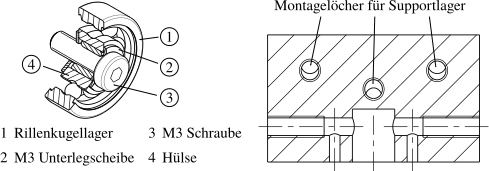
\includegraphics[]{./images/kugelsupport.pdf}
    \caption{Das Supportlager (links) und der Kunststoffsockel (rechts)}
    \label{fig:das_modifizierte_kugelsupport}
\end{figure}
%

Der Kohlebürstenhalter ist aus Messing, hat eine zylindrische Form und wird mit einem Blechhalter, welcher an der Seite des Supports angeschraubt wird, gelötet.
Die Kohlebürste Typ \textit{KK399} wurden von der Firma \textit{Schmidthammer} gekauft.
Dank dem hohen Kupferanteil (98\%) hat sie sehr geringen Kontaktwiderstand bzw. Eigenwiderstand.
Sie hat am Ende eine Kupferlitze und ist an anderen Seite mit Laufschräge zu versehen.
Leider ist die Laufschräge für diese Anwendung nicht geeignet und wurden flach geschliffen.
Die Kohlebürste wird von einer Feder (Typ \textit{LG860}) gegen der Lauffläche (Kugelaufnahme) gedrückt.
Abbildung \ref{fig:die_baugruppe_des_kohlebuerstenhalters} zeigt die Baugruppe des Kohlebürstenhalters.
% ----------------------------------------
% Fig: Blechhalter + Kohlebürstenhalter + Kohlebürsten + Feder
% ----------------------------------------
\begin{figure}[htb]
    \centering
    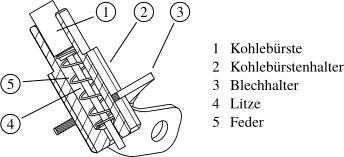
\includegraphics[]{./images/kohlebuerstenhalter_asm.pdf}
    \caption{Die Baugruppe des Kohlebürstenhalters}
    \label{fig:die_baugruppe_des_kohlebuerstenhalters}
\end{figure}
%

Um der elektrische Kontakt zwischen der Kugel und der Messprobe während der Versuche geringe Störungen zu halten, sind zwei Kohlebürsten für die Kugel zu versehen.
Abbildung \ref{fig:das_komplette_kugelsupports} zeigt das komplette Supports mit der neuen Kugelführung.
% ----------------------------------------
% Fig: Zusammenbau des gesamten Kugelsupports
% ----------------------------------------
\begin{figure}[htb]
    \centering
    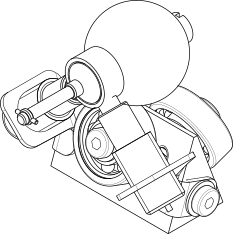
\includegraphics[]{./images/kugelsupport_full.pdf}
    \caption{Zusammenbau des neuen Supports mit der Kugel}
    \label{fig:das_komplette_kugelsupports}
\end{figure}
%

% ----------------------------------------
% Sec: Die Glasscheibebaugruppe
% ----------------------------------------
\section{Die Glasscheibebaugruppe}
\label{sec:die_glasscheibebaugruppe}

Um die elektrische Messung bei dem vorhandenen Prüfstand durchzuführen, müssen die folgende Maßnahmen gemacht werden:
\begin{itemize}
    \item Stromleitende Beschichtung für die Glasscheibe
    \item Isolierung der Glasscheibe mit dem gesamten Prüfsystem
    \item Elektrischer Zugang für die Messprobe zur Unterseite der Glasscheibe
\end{itemize}

Wie im vorherigen Kapitel \ref{chap:literaturforschung_der_experimentellen_technik_in_ehd_schmierung} schon erwähnt, ist es auch möglich, die Schmierfilmdickenmessung bei einer Chrom beschichteten Scheibe durch zu führen.
Allerdings es gibt folgende Probleme bei der klassischen Messmethode.
Ersten bietet dieses Verfahren eine niedrige Auflösung. Zweiten ist eine monochrom Lichtquelle notwendig, es fehlt bei dem vorhandenen Prüfstand diesen Apparat.
Nicht zuletzt ist das \textit{Ultra-Softwarepaket} von PCS nicht in der Lager solche Messung durchzuführen bzw. auszuwerten.
Letzten ist der Eigenwiderstand der Chromschicht wegen ihrer extrem dünnen Dicke sehr hoch (größer als $1 \ k\Omega$).
\label{chap:literaturforschung_der_experimentellen_technik_in_ehd_schmierung}
Das macht die optische und elektrische Messung bei der Chrom-Glasscheibe ungünstig.

Eine andere Option ist die \textit{Spacer-Layer-Scheibe} zu benutzen.
Da die Silikatschicht nicht Strom leitend ist, wird die Hälfte der Scheibe mit einer dickeren Chromschicht (c.a $300 \ nm$) beschichtet (Abbildung \ref{fig:die_neu_beschichtet_glassscheibe}).
Durch die Erhöhung der Beschichtungsdicke wird der Eigenwiderstand reduziert.
Ein paar Widerstandsmessung mit einem Multimeter lieferten den maximalen Wert von $8 \ \Omega$ und den minimalen Wert von $2,4 \ \Omega$.
Die unbehandelte Hälfte kann man wie normal mit der \textit{Spacer-Layer-Methode} benutzen, um die Schmierfilmdicke zu bestimmen.
% ----------------------------------------
% Fig: Bild der neuen beschichteten Scheibe
% ----------------------------------------
\begin{figure}[htb]
    \centering
    \includegraphics[]{./images/beschichtete_scheibe.pdf}
    \caption{Die neue Spacer-Layer-Glasscheibe mit sichbarer beschichteten Hälfte}
    \label{fig:die_neu_beschichtet_glassscheibe}
\end{figure}
%

Der nächste Schritt ist die behandelte Glasscheibe mit dem gesamten Testsystem isolieren.
Das erfolgt durch die Verwendung einer Kunststoff-Unterlegscheibe und einer Kunststoffhülse, die Unterseite der Scheibe mit der Welle des 1. Motors trennen (Abbildung \ref{fig:isolierung_der_glassscheibe})
Beide Teile sind aus \textit{Polypropylen}, welcher bis $80 ^\circ C$ beständig ist und die Unterlegscheibe ist nur $0,5 mm$ dick.
Da die Lasteinheit nicht nur in die horizontale sondern auch in die vertikale Richtung sich bewegen kann, ist diese minimale Höheänderung der Glasscheibe kein Problem.
Die äußere Oberfläche der Hülse wurden an sechs Positionen flach gefräst. Die bilden sich mit der inneren Bohrung der Glasscheibe sechs Kanäle, die den Platz für die elektrische Verbindungen von Unterseite zur Oberseite der Scheibe schaffen.
Die Kunststoff-Unterlegscheibe wurde mit der Hülse mit dem \textit{Plastix} Klebe von Pattex geklebt, diese Verbindung ist gegen dem Wegrutschen der beiden Teilen während Betriebs zu sichern.
% ----------------------------------------
% Fig: Isolierung der Scheibe
% ----------------------------------------
\begin{figure}[htb]
    \centering
    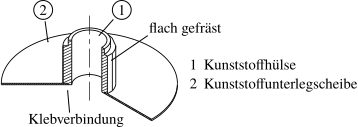
\includegraphics[]{./images/isolierung_der_scheibe.pdf}
    \caption{Isolierung der Glasscheibe}
    \label{fig:isolierung_der_glassscheibe}
\end{figure}
%

Um die elektrische Verbindung von der Unterseite der Scheibe nach oben zu bringen, werden sechs Kupferstreifen verwendet.
Sie werden auf der Kunststoff-Unterlegscheibe angeklebt und durch die sechs Kanäle (zwischen Hülse und Glasscheibe) nach oben geführt.
Dort werden sie bei der Montageposition zwischen der Oberkante der Hülse und einer Mitnehmerscheibe geklemmt und dadurch ist die elektrische Verbindung zwischen beiden Seite Scheibe hergestellt.
Die von oben geschraubt Sicherungsmutter sichert die ganze Baugruppe fest.
Die Abbildung \ref{fig:glasscheibebaugruppe} zeigt die ganze Baugruppe der Glasscheibe an.
% ----------------------------------------
% Fig: Glasscheibebaugruppe
% ----------------------------------------
\begin{figure}[htb]
    \centering
    \includegraphics[width=4cm]{./images/blank_img.jpg}
    \caption{Glasscheibebaugruppe}
    \label{fig:glasscheibebaugruppe}
\end{figure}
%

% ----------------------------------------
% Sec: Konstruktion des Deckels
% ----------------------------------------
\section{Konstruktion des Deckels}
\label{sec:konstruktion_des_deckels}

Der originale Deckel des EHD-Prüfstands von PCS hat zwei wichtige Aufgabe.
Erste soll er das Spritzöl vom Ölreservoir auf der Oberseite der Glasscheibe und in die Linsen der Lichtquelle schützen.
Zweite, da es nur eine Öffnung für die Lichtquelle auf dem Deckel gibt, soll er die Störungen wegen Streulicht aus der Umgebung in den EHD-Kontakt bei der Messung reduzieren.

Für diese Arbeit wurde der Deckel modifiziert, so dass man die Kohlebürste, die die Messignale von der Glasscheibe aufnimmt, in dem Deckel integrieren kann.
Die gesamte Kohlebürste-Baugruppe wurde in dem Deckel durch eine $M8$ Bohrung angeschraubt und durch eine Kontermutter in Position gesichert.
Dadurch wird die elektrische Kontakt zwischen der Kohlebürste und der Glasscheibe über die Mitnehmerscheibe hergestellt.
An der Kante des Deckels gibt es eine kleine gefräste Nut.
Durch die werden die von der Kugel zu tragenden Messignalen Leitungen nach draußen an dem Messgerät geführt.
Abbildung \ref{fig:deckel_mit_kohlebuersten} zeigt den neuen Deckel und den elektrischen Kontakt zwischen der im Deckel integrierten Kohlebürste und der Glasscheibe.
% ----------------------------------------
% Fig: Der neue Deckel
% ----------------------------------------
\begin{figure}[htb]
    \centering
    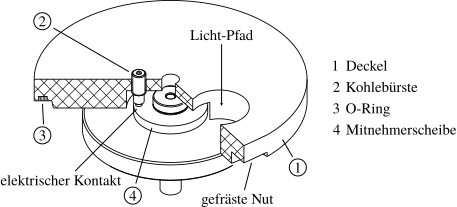
\includegraphics[]{./images/deckel_und_scheibe.pdf}
    \caption{Der neue Deckel mit der integrierten Kohlebürste}
    \label{fig:deckel_mit_kohlebuersten}
\end{figure}
%


% ----------------------------------------
% Versuche beim EHD-Messgerät
% ----------------------------------------
% ----------------------------------------
% Chap: Versuche auf dem EHD-Messgerät
% ----------------------------------------
\chapter{Versuche auf dem EHD-Messgerät}
\label{chap:versuche_auf_dem_ehd_messgeraet}

\improvement[inline]{Sagen, dass die Schmierfilmdickenmessung auch mit optisch ausgeführt wird.}

% ----------------------------------------
% Sec: Kapazitive Messgeräte zur Schmierfilmdickenbestimmung
% ----------------------------------------
\section{Kapazitive Messgeräte zur Schmierfilmdickenbestimmung}
\label{sec:kapazitive_messgeraete_zur_schmierfilmdickenbestimmung}

% ----------------------------------------
% Sub: Stromladekurve Messgerät
% ----------------------------------------
\subsection{Stromladekurve Messgerät}
\label{sub:stromladekurve_messgeraet}

Im IMKT gibt es ein mobiles Messsystem zur Schmierfilmdickenmessung mittels kapazitiven Messverfahren.
Das System besteht aus einem Laptop, der mit \textit{Laderkurve-Software} installiert, und einer Messkarte (Typ USB-6211) von der Firma National Instrument (NI).

Bei kapazitiver Messmethode wird der EHD-Kontakt als ein Kondensator ($C_K$) betrachtet.
Die Auflade des Kondensators erfolgt durch eine Ladespannung $U_L$ (\SIrange{0,2}{0,5}{\volt}) und einen Vorwiderstand $R_V$ (\SI{1012.7}{\kilo\ohm}).
Eine unendliche Erhöhung der Ladespannung ist aber unerwünscht, weil die zur Ionisierung des Schmierstoffes bei hohen Spannung verursacht und das kann die Messergebnisse verfälschen.
Abbildung \ref{fig:Schematischer_aufbau_des_mobilen_messsystems} zeigt das Prinzip des mobilen Messsystems zur Schmierfilmdickenmessung bei IMKT an.
% ----------------------------------------
% Fig: Schematischer Aufbau des mobilen Messsystems
% ----------------------------------------
\begin{figure}[htb]
    \centering
    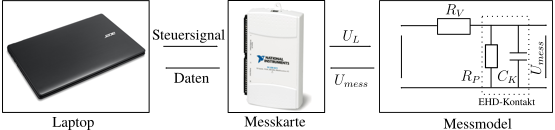
\includegraphics[]{./images/schematischer_aufbau_des_mobilen_messsystem.pdf}
    \caption{Schematischer Aufbau des mobilen Messsystems}
    \label{fig:Schematischer_aufbau_des_mobilen_messsystems}
\end{figure}

Das ganze Messsystem wird von der \textit{Laderkurve-Software} gesteuert.
Sie miss nicht direkt die Kapazität, sondern nimmt sie die Antwort bzw. Ladekurve des ``Kondensators'' auf, danach wird die Auswertung mit einem Matlab-Skript ausgeführt.
Die Software kann die Ladekurve in zwei Modi: \emph{Anzahl der Messwerte} oder \emph{Messung nach Zeit} aufnehmen.
Im Rahmen dieser Arbeit werden alle Messungen mit dem ersten Modus gemacht.
Abbildung \ref{fig:gui_der_laderkurve_software} zeigt die Benutzeroberfläche der Ladekurve-Software bei einer Testmessung mit einem Referenz-Kondensator (\SI{3.3}{\nano\farad}) an.
% ----------------------------------------
% Fig: GUI der Ladekurve-Software
% ----------------------------------------
\begin{figure}[htb]
    \centering
    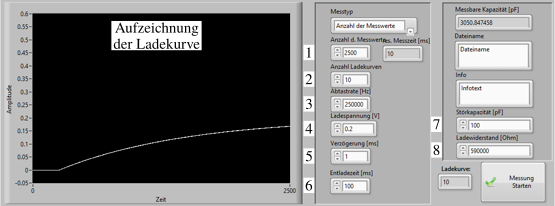
\includegraphics[]{./images/ladekurven_gui.pdf}
    \caption{Benutzeroberfläche der Laderkurve-Software}
    \label{fig:gui_der_laderkurve_software}
\end{figure}

Die Software ist relative einfach zu bedienen, allerdings gibt es folgende Punkte, auf die man beachten muss.
\begin{description}
    \item[1. Anzahl der Messwerte] ist die Auflösung der Messung.
        Zu niedriger Wert kann zum Messfehler führen und zu hohen Wert kann es schnell den Speicher voll machen, außerdem ist sie auch von der Abtastrate der Messkarte beschränkt.
        Der Standardwert ist \num{2500}.

    \item[2. Anzahl der Ladekurven] ist die Anzahl der Messungen, die nach einander durchgeführt werden. ist die Anzahl der Messungen, die nach einander durchgeführt werden.
        Der Standardwert ist \num{10}.

    \item[3. Abtastrate] ist die Anzahl der Messwerte, die Messkarte pro Sekunde messen kann.
        Die USB-6211 Messkarte von NI kann maximal \SI[per-mode=symbol]{250}{\kilo\sample\per\second}, das entspricht \num{2500} Messwerte in einem Zeitraum von \SI{10}{\milli\second}.

    \item[4. Ladespannung] ist die Spannung zwischen zwei Terminal des Kondensators.
        Der Wert sollte im Bereich von \SIrange{0.2}{0.5}{\volt} liegen.

    \item[5. Verzögerung] ist die Wartezeit, die die Software warten muss, bevor sie eine Messung ausführt.
        Der Standardwert ist \SI{1}{\ms}.

    \item[6. Entladezeit] ist die Zeit zwischen zwei Messungen.
        Sie ist notwendig, um der Kondensator komplette leer bevor jeder neuen Messung zu entladen.
        Der Standardwert ist \SI{100}{\ms}.

    \item[7. Ladewiderstand] ist der Wert des Vorwiderstands.
        Er ist nur für den Dokumentationszweck und wird in der Messdatei geschrieben.

    \item[8. Störkapazität] ist die externe Störung, wie zum Beispiel von Messkabel oder statische Kapazität zwischen Messkörpern.
        Dieser Wert wird für die spätere Auswertung verwendet.

    \item[9. Austecken des Netzteils] ist notwendig, um die Störungen von anderen elektronischen Geräte zu vermeiden.
\end{description}

%
% ----------------------------------------
% Sub: LCR Messgerät
% ----------------------------------------
\subsection{LCR Messgerät}
\label{sub:lcr_messgeraet}

In der Praxis kann jede Flüssigkeit und jeder Feststoff Strom durchlassen.
Wenn das Material von einem Wechselstrom gespeist wird, wird das Verhältnis zwischen der Spannung und dem Strom als Impedanz bezeichnet.
Die Veränderung der gemessenen Impedanz durch die Variation der Stromfrequenz ist von der Eigenschaft des Materials abhängig.
Das kann auf die physikalische Struktur des Werkstoffes, auf die innere chemische Prozesse oder eine Kombination von beiden zurückführen.
Der Zusammenhang zwischen der Impedanz, der Frequenz und der Kapazität von einem mit Wechselstrom angelegten Kondensators wird in der Formel \ref{eq:impedanz_kondensator} \cite{impedance} dargestellt.
%
\begin{equation}
    Z_{C} = \cfrac{v_C(t)}{i_C(t)} = \cfrac{1}{j \omega C}
    \label{eq:impedanz_kondensator}
\end{equation}

Im Gegenteil zum mobilen Ladekurve-Messsystem, welches die Kapazität über die Antwort einer Ladespannung interpretiert, bietet das LCR-Messgerät ST2826 der Firma Sourcetronic die Möglichkeit, die Kapazität eines EHD-Kontakts direkt zu messen.
Abbildung \ref{fig:versuchsaufbau_zur_kapazitaetsmessung_mit_lcr_meter} zeigt den Aufbau des Messsystems mit dem LCR-Messgerät.
% ----------------------------------------
% Fig: Schematischer Aufbau des Messsystems mit LCR-Meter
% ----------------------------------------
\begin{figure}[htb]
    \centering
    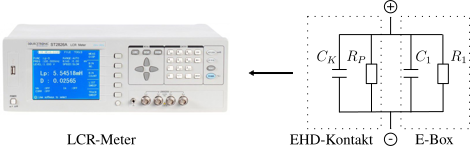
\includegraphics[]{./images/versuchsaufbau_mit_lcr_meter.pdf}
    \caption{Versuchsaufbau zur Kapazitätsmessung mit LCR-Meter}
    \label{fig:versuchsaufbau_zur_kapazitaetsmessung_mit_lcr_meter}
\end{figure}

Das LCR-Messgerät bietet einen breiten Frequenzbereich von \SI{20}{\Hz} bis \SI{50}{\MHz}.
Dank der Kelvin-Messproben (4-Punkt Messung) hat das Gerät eine sehr gute Genauigkeit von \SI{0.1}{\percent} und ermöglicht die Messung auch bei kleinsten Änderung des Systems.
Mit einer Sinuskorrelationstechnik bietet das Gerät eine rauschfreie Analyse.
Die Addition des Widerstands $R_1$ und des Kondensators $C_1$ sind benötigt, um zu sehen, ob der Strom tatsächlich durch den EHD-Kontakt fließt oder in irgeneiner Verbindung verloren geht.
Unterschiedliche Werte für $R_1$ und $C_1$ wurden verwendet, um deren Einfluß auf die gemessene Kapazität zu untersuchen.
Ein Erhöhung des Widerstandswertes führt zu einer signifikanten Abnahme der Messergebnisse und umgekehrt.
Dieses Phänomen kann durch die Abnahme bzw. Zunahme des Stromflusses durch den EHD-Kontakt erklärt werden.
Die Werte $R_1 = 2$ \si{\kilo\ohm} und $C_1 = 24$ \si{\pico\farad} wurden durch Experiment für weitere Messungen in dieser Arbeit gewählt.
Abbildung \ref{fig:messprobe_eines_mit_dem_lcr_meter} zeigt das Messergebnis beim Referenz-Kondensator (\SI{3.3}{\nano\F}) mit dem LCR-Messgerät bei verschiedenen Frequenzen.
% ----------------------------------------
% Fig: Messprobe mit 24 pF mit dem LCR-Meter
% ----------------------------------------
\begin{figure}[htb]
    \centering
    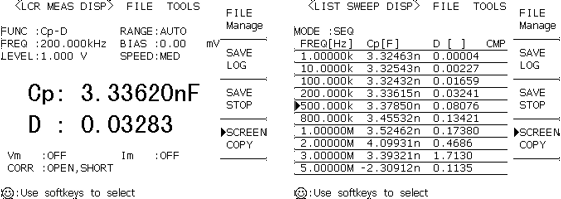
\includegraphics[]{./images/messprobe_mit_lcr_meter.pdf}
    \caption{Messergebnis eines Referenz-Kondensators mit dem LCR-Messgerät}
    \label{fig:messprobe_eines_mit_dem_lcr_meter}
\end{figure}

\improvement[inline]{Update the measurements LCR-Meter}

% ----------------------------------------
% Sec: Versuchdurchführung
% ----------------------------------------
\section{Versuchdurchführung}
\label{sec:versuchdurchfuehrung}
\improvement[inline]{Schreiben der Versuchdurchführung}

In dieser Arbeit werden die Versuche mit dem Versuchsöl \textit{FVA3} wie folgt geplant:
% ----------------------------------------
% Enum: Versuchsplan
% ----------------------------------------
\begin{enumerate}
    \item Vergleichsmessungen von neu modifizierten Bauteilen (Kugel, Support, Glasscheibe) mit den von \textit{PCS}
    \item Schmierfilmdickenmessung am EHD-Gerät (optisch)
    \item Schmierfilmdickenmessung mit dem mobilen Messsystem von IMKT (elektrisch)
    \item Vergleich der theoretischen Schmierfilmdickenbestimmung mit 2. und 3. zur Überprüfung des Messverfahrens
\end{enumerate}

Da die Auswertung der Schmierfilmdicke in dieser Arbeit optisch und elektrisch geschieht wird, ist die Sauberkeit vor dem Beginn einer Messung besonders wichtig zu achten.
Die Glasscheibe, die Kugel, das Kugelsupport und das Ölreservoir müssen vor jeder Messung mit Waschbenzin oder Isopropanol gereinigt werden und dürfen keine Schlieren aufweisen.
Nach der Reinigung können das Support und die Kugel in das Gerät eingesetzt werden.
Die Führung der Kugel wird zuerst in die Ausgangswelle des zweiten Motors eingesteckt und dann auf das Support aufgelegt.
Die Kabel sollen Abstand von den Wände des Reservoirs und der Motorwelle gehalten werden, um ein Unfall (Kurzschluss der Kugel, Verfangen des Kabels) während des Betriebs zu vermeiden.
Die Abbildung \ref{fig:ehd_topf_mit_kugel_und_support} zeigt den Blick von oben des EHD-Prüftopfs mit montierten Support und aufgelegter Kugel bereits für den Versuch.
% ----------------------------------------
% Fig: EHD-Prüftopf mit montierten Support und Modifizierter Kugelführung
% ----------------------------------------
\begin{figure}[htb]
    \centering
    \includegraphics[width=0.8\linewidth]{./images/ehd_topf_mit_kugel_und_support.jpg}
    \caption{Topf des EHD-Geräts mit montierten neuen Kugelsupport und der Modifizierter Kugelführung}
    \label{fig:ehd_topf_mit_kugel_und_support}
\end{figure}

Der Widerstand der gesamten Messkette (Kabel -> Scheibe -> Kugel -> Kabel) wird vor jedem Versuch im Stillstand unter einer Last von \SI{20}{\newton} vermessen und er betrug zwischen \SIrange{17}{18}{\ohm}.
Neben dem Widerstand wird die Hintergrund-Kapazität des Prüfstands auch gemessen, weil dieser Wert als Störkapazität bezeichnet wird und soll von der Ergebnissen beseitigt werden.

Die Last von \SI{20}{\newton} wird in Anlehnung an vorherigen Arbeiten gewählt.
Nach dem Abschnitt \ref{sec:betrachtung_des_ehd_kontaktes} lässt es sich für den hier betrachteten Fall eines Kugel-Scheibe-Modells eine maximale Pressung im Kontakt $p_0 =$ \SI{505}{\mega\pascal} berechnen.
Damit liegt der Kontakt im unteren Bereich der EHD-Schmierung.
Diese geringe Last ist gut, somit wird die Gefahr von Beschädigung auf der Scheibe bzw. der Silikatschicht gering gehalten.

Zur Messung bei Öl-Vollschmierung wird das Ölreservoir bis zur Hälfte der Kugel (ca. \SI{120}{\ml}) gefüllt.
Das Ölbad wird vor jeder Messreihe während des Heizvorgangs (bei \SI{40}{\degreeCelsius}, \SI{60}{\degreeCelsius} und \SI{80}{\degreeCelsius}) für ca. \SI{10}{\minute} durchmischt, um eine homogene Temperatur im Ölbad beim Versuch zu herrschen.
Das genaue Vorgehen einer solchen Messung wurde von \textit{Surborg} in seiner Arbeit \cite{surborg_2007} beschrieben und ist im Anhang zu finden.

Die Versuchparameter aller Messungen in dieser Arbeit werden in der Tabelle \ref{tab:ehd_test_params} zusammengefasst.
% ----------------------------------------
% Tab: Versuchsparameters am EHD-Prüfstand
% ----------------------------------------
\begin{table}[htbp]
    \centering
    \caption{Versuchsparameters beim EHD-Prüfstand}
    \begin{tabular}{ll}
        Öl & FVA 3 \\
        Last [\si{N}] & 20 \\
        Temperatur [\si{\degreeCelsius}] & 40 – 60 – 80 \\
        Geschwindigkeit [\si[per-mode=symbol]{\meter\per\second}] & \SIrange[per-mode=symbol]{0.02}{4}{\meter\per\second} \\
        Geschw. Stufen [\si{\%}] & 20 \\
        Schlupf [\si{\%}] & 5 \\
    \end{tabular}
    \label{tab:ehd_test_params}
\end{table}




% ----------------------------------------
% Diskussion
% ----------------------------------------
\chapter{Diskussion}
\label{chap:diskussion}


% ----------------------------------------
% Zusammenfassung und Ausblick
% ----------------------------------------
\chapter{Zusammenfassung und Ausblick}
\label{zusammenfassung_und_ausblick}

Was soll in die Zusammenfassung sein.

Was ist der Ausblick von dieser Arbeit


% ----------------------------------------
% Literaturverzeichnis
% ----------------------------------------
\bibliographystyle{unsrt}
\bibliography{./literatures/literaturen}

% ----------------------------------------
% Anhang
% ----------------------------------------
\begin{appendix}
Bilde, Formelherleitung, Zeichnung etc...
\end{appendix}


\end{document}
